\section{Javascript}

\subsection{Explosion of Javascript popularity}

\subsubsection{In the beginning}

Javascript was created by Brendan Eich at Netscape around May 1995, and released to the public in September.
The initial name of the project was Mocha, then LiveScript, the name Javascript was finally adopted to leverage the trend around Java.
The latter was considered the hot new web programming language at this time.
It was quickly adopted as the main language for web servers, and everybody was betting on pushing Java to the client as well.
The history proved them wrong.
% Javascript slowly took over the client, and is now pushing toward the server.
% But that was not a calm and linear journey.

In 1995, when Javascript was released, the world wide web started its wide adoption.\ftnt{http://www.internetlivestats.com/internet-users/}
Browsers were emerging, and started a battle to show off the best features and user experience to attract the wider public.\footnote{to get an idea of the web in 1997 : \url{http://1x-upon.com/}}
Microsoft released their browser Internet Explorer 3 in June 1996 with a concurrent implementation of Javascript.
They changed the name to JScript, to avoid trademark conflict with Oracle Corporation, who owns the name Javascript.
The differences between the two implementations made difficult for a script to be compatible to both.
At the time, signs started to appear on web pages to warn the user about the ideal web browser to use for the best experience on this page.
This competition was fragmenting the web.
% and the overall user experience could be improved by /// according the technology ///.

To stop this fragmentation, Netscape submitted Javascript to Ecma International for standardization in November 1996.
In June 1997, ECMA International released ECMA-262, the first specification of ECMAScript, the standard for Javascript.
A standard to which all browser should refer for their implementations.
% TODO more on the Ecma specification ?

The base for this specification was designed in a rush. The version released in 1995 was finished within 10 days.
Because of this precipitation, the language has often been considered poorly designed and unattractive.
Moreover, Javascript was intended to be simple enough to attract unexperienced developers, by opposition to Java or C++, which targeted professional developers.
For these reasons, Javascript started with a poor reputation among the developer community.

But things evolved drastically since.
When a language is released, available freely at a world wide scale, and simple enough to be handled by a generation of teenager inspired by the technology hype, it produce an effervescent community around what is now one of the most popular and widely used programming language.

\subsubsection{Rising of the unpopular language}

Javascript started as a programming language to implement short interactions on web pages.
The best usage example was to validate some forms on the client before sending the request to the server.
This situation hugely improved since the beginning of the language.
So much that web-based, Javascript applications are currently now favored instead of rich, native desktop applications.

ECMA International released several version in the few years following the creation of Javascript.
The first and second version, released in 1997 and 1998, brought minor revisions to the initial draft.
However, the third version, released in the late 1999, contributed to give Javascript a more complete and solid foundation as a programming language.
From this point on, the consideration for Javascript keep improving.

An important reason for this reconsideration started in 2005.
James Jesse Garrett released \textit{Ajax: A New Approach to Web Applications}, a white paper coining the term Ajax \cite{Garrett2005}.
This paper point the trend in using this technique, and explain the consequences on user experience.
Ajax stands for Asynchronous Javascript And XML.
It consists of using Javascript to dynamically request and refresh the content of a web page.
The advantage is that it avoids to request a full page from the server.
Javascript is not anymore confined to the realm of small user interactions on a terminal, it can be proactive and responsible for a bigger part in the system spanning from the server to the client.
Indeed, this ability to react instantly to the user started to narrow the gap between web and native applications.
%, while keeping all the advantages of web-based applications.
At the time, the first web applications to use Ajax were Gmail, and Google maps\footnote{A more in-depth analysis of the history of Ajax, given by late Aaron Swartz \url{http://www.aaronsw.com/weblog/ajaxhistory}}.

Around this time, the Javascript community started to emerge.
The third version of ECMAScript had been released, and the support for Javascript was somewhat homogeneous on the browsers but far from perfect.
Moreover, Javascript is only a small piece in the architecture of a web-based client application.
The DOM, and the \texttt{XMLHttpRequest} method, two components on which AJAX relies, still present heterogeneous interfaces among browsers.
To leverage the latent capabilities of Ajax, and more generally of the web, Javascript framework were released with the goal to straighten the differences between browsers implementations.
Prototype\ftnt{http://prototypejs.org/} and DOJO\ftnt{https://dojotoolkit.org/} are early famous examples, and later jQuery\ftnt{https://jquery.com/} and underscore\ftnt{http://underscorejs.org/}.
These frameworks are responsible in great part to the wide success of Javascript and of the web technologies.

In the meantime, in 2004, the Web Hypertext Application Technology Working Group\ftnt{https://whatwg.org/} formed to work on the fifth version of the HTML standard.
This new version provide new capabilities to web browsers, and a better integration with the native environment.
It features geolocation, file API, web storage, canvas drawing element, audio and video capabilities, drag and drop, browser history manipulation, and many mores
It gave Javascript the missing pieces to become a true language for developing rich application.
The first public draft of HTML 5 was released in 2008, and the fifth version of ECMAScript was released in 2009.
With these two releases, ECMAScript 5 and HTML5, it is a next step toward the consideration of Web-based technologies as equally capable, if not more, than native rich applications on the desktop.
Javascript became the programming language of this rising application platform.

However, if web applications are overwhelmingly adopted for the desktop, HTML5 is not yet widely accepted as ready to build complete application on mobile, where performance and design are crucial.
Indeed web-technologies are often not as capable, and well integrated as native technologies.
But even for native development, Javascript seems to be a language of choice.
An example is the React Native Framework\ftnt{https://facebook.github.io/react-native/} from Facebook, which allow to use Javascript to develop native mobile applications.
They prone the philosophy \textit{"learn once, write anywhere"}, in opposition to the usual slogan \textit{"write once, run everywhere"}.\footnote{Used firstly by Sun for Java, but then stolen by many others}
% Another example is Gnome-shell. It uses Javascript to build its interface, and extensions.
% PhoneGap (Cordova) is a huge effort toward bringing web technologies to the mobile. 

\subsubsection{Current situation}

\cit{When JavaScript was first introduced, I dismissed it as being not worth my attention. Much later, I took another look at it and discovered that hidden in the browser was an excellent programming language.}{Douglas Crockford}

% \cit{JavaScript is the world's most ubiquitous computing runtime.}{John Lam}

The success of Javascript is due to many factors ; I mentioned previously the standardization, Ajax libraries and HTML5.
Another factor, maybe the most important, is the View Source menu that reveals the complete source code of any web application.
\textit{The view source menu is the ultimate form of open source}\ftnt{http://blog.codinghorror.com/the-power-of-view-source/}.
It is the vector of the quick dissemination of source code to the community, which picks, emphasizes and reproduces the best techniques.
This brought open source and collaborative development before github. \comment{TODO neither open source nor collaborative development are the correct terms}
Moreover, all modern web browsers now include a Javascript interpreter, making Javascript the most ubiquitous runtime in history \cite{Flanagan2006}.
% Every browser include development tools for Javascript, making it the most ubiquitous development environment, as well.

When a language like Javascript is distributed freely with the tools to reproduce and experiment on every piece of code.
When this distribution is carried during the expansion of the largest communication network in history.
Then an entire generation seizes this opportunity to incrementally build and share the best tools they can.
This collaboration is the reason for the popularity of Javascript on the Web.

% I want to say that Javascript took off because it was carried by the open source community.
% The goal is to introduce the following facts : JS is widely used in the open source community.
% I need to find the argument saying that open source is taking over closed sources : Javascript / open source is taking over Java / closed source.

% TO READ :
% http://www.javaworld.com/article/2077224/learn-java/is-javascript-here-to-stay-.html
% http://blog.codinghorror.com/the-power-of-view-source/
% http://blog.codinghorror.com/javascript-the-lingua-franca-of-the-web/
% http://shaver.off.net/diary/2007/05/10/the-high-cost-of-some-free-tools/


% This success is obvious on the web and in the open source communities.
It seems to also infiltrate many other fields of IT, but it is hard to give an accurate picture of the situation.
There is no right metrics to measure programming language popularity.
In the following paragraphs, I report some popular metrics and indexes available on the net.
More detailed informations are available section \ref{appendix:langpop}.

\paragraph{Search engines}

The TIOBE Programming Community index is a monthly indicator of the popularity of programming languages.
It uses the number of results on many search engines as a measure of the activity of a programming language.
Javascript ranks 6th on this index, as of April 2015, and it was the most rising language in 2014.
However, the measure used by the TIOBE is controversial.
Some says that the measure is not representative.
It is a lagging indicator, and the number of pages doesn't represent the number of readers.

On the other hand, the PYPL index is based on Google trends to measure the activity of a programming language.
Javascript ranks 7th on this index, as of May 2015.

From these indexes, the major programming languages are Java, C/C++ and C\#.
The three languages are still the most widely taught, and used to write softwares.
But Javascript is rising to become one of these important languages.

\paragraph{Developers collaboration platforms}

Github is the most important collaborative development platform, with around 9 millions users.
Javascript is the most used language on github since mid-2011, with more than 320 000 repositories.
The second language is Java with more than 220 000 repositories.

\comment{TODO : graph of Github repositories by languages}

StackOverflow, is the most important Q\&A platform for developers.
It is a good representation of the activity around a language.
Javascript is the second language showing the most activity on StackOverflow, with more than 840 000 questions.
The first one is Java with more than 850 000 questions.

Black Duck knowledgebase analyzes 1 million repositories over various forges, and collaborative platforms to produce an index of the usage of programming language in open source communities.
Javascript ranks second.
C is first, and C++ third.
Along with Java, the four first languages represent about 80\% of all programming language usage.

% TODO redo this graph, it is ugly.
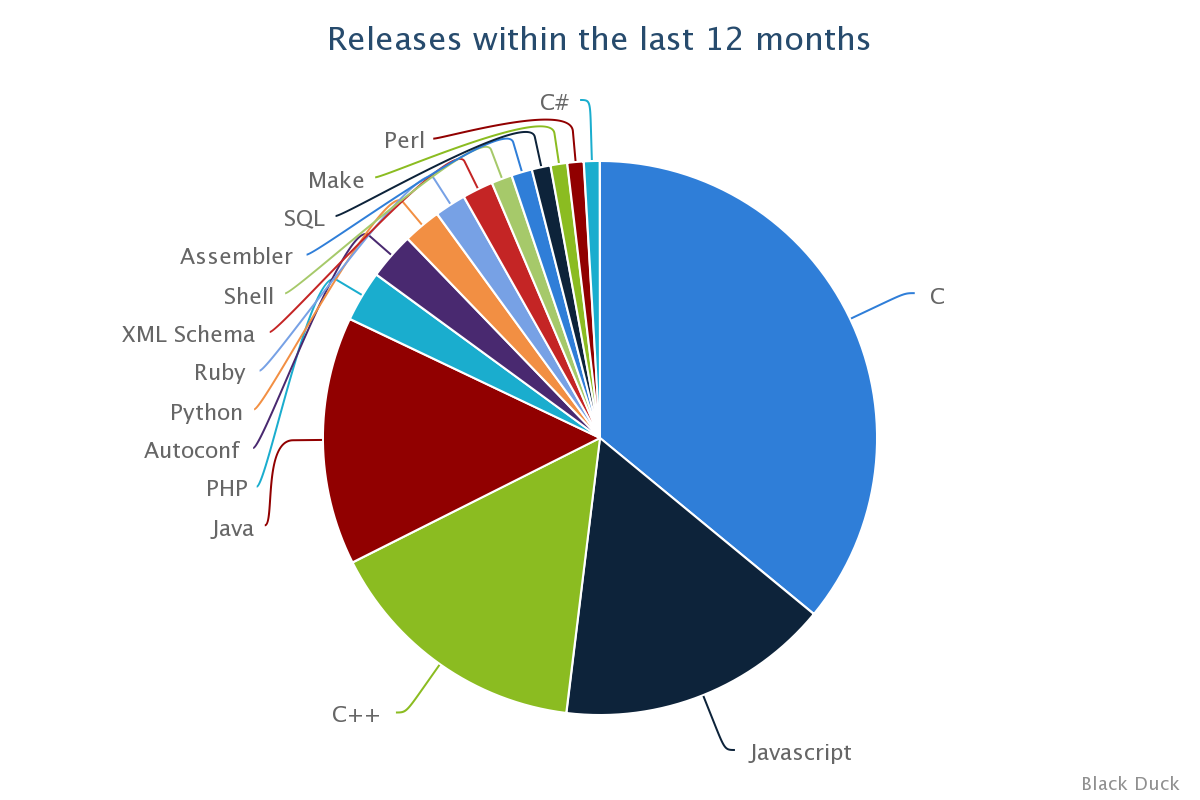
\includegraphics[width=0.9\linewidth]{../../data/js-trends/black-duck-15}

\paragraph{Jobs}

All these metrics are representing the visible activity about programming language.
But not the entire software industry is open source, and the activity is rather opaque.
To get a hint on the popularity of programming languages used in the software industry, let's look at the job offerings.
Indeed provide some insightful trends.
Javascript developers ranked at the third position, right after SQL developers and Java developers.
Then come C\# and C developers.

% TODO redo this graph, it is ugly.
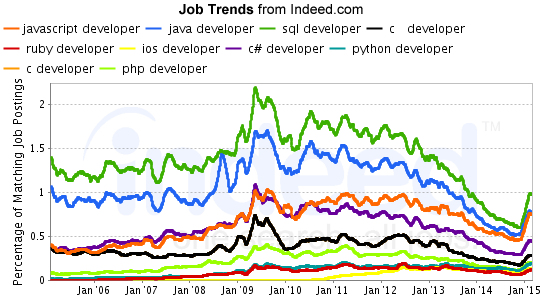
\includegraphics[width=0.9\linewidth]{../../data/js-trends/jobgraph}

All these metrics represent different faces of the current situation of Javascript adoption.
We can safely say that Javascript is one of most important language of this decade, along with Java, C/C++.
It is widely used in open source projects, and everywhere on the web.
But it is also trending, and maybe slowly replacing languages like Java.
% TODO continue this

\paragraph{Future trends}

\comment{TODO}

Code reuse.
Why it never worked ?




\comment{em-scripten}

https://github.com/kripken/emscripten
Javascript is a target language for LLVM, therefor everything can compile to Javascript : JS is the assembler of the web.

\comment{Isomorphic Javascript}

Server-side Javascript

https://www.meteor.com/
https://facebook.github.io/flux/
Javascript can be executed both on the client and the server.
That allow use-cases never possible before (server pre-rendering, same team ...)

\comment{Reactive}

http://facebook.github.io/react/
Javascript is used to model the flow of propagation of state in a web application



---

Some facts to include :
https://www.destroyallsoftware.com/talks/the-birth-and-death-of-javascript
The Atom editor is written in Javascript node.js.
Now, major PaaS (which one) support node.js by default.
Heroku support Python, Java, Ruby, Node.js, PHP, Clojure and Scala
Amazon Lambda Web service support node.js in priority.
npm raises 8m.
http://techcrunch.com/2015/04/14/popular-javascript-package-manager-npm-raises-8m-launches-private-modules/

% >>> I want to say that Javascript is now broadly used.
% Let's just look at the numbers : Javascript is the most popular language on Github, and npm has more package than any other package manager.
% Javascript has the more broadly deployed runtime.
% ... and so on
% >>> the conclusion is : Javascript is now a major language, and it is more than worth the consideration we are giving it in this PhD thesis.

\subsection{Overview of the language}

Javascript was released in a hurry, without a strong and directive philosophy.
During its evolution, it snowballed with different features to accommodate the community, and the usage it was made on the web. As a result Javascript contains various, and sometimes conflicting, programming paradigms.
It borrow its syntax from a procedural language, like C, and the object notation from an object-oriented language, like Java, but it provides a different inheritance mechanism, based on prototypes. Most of the implementation adopt an event-based paradigm, like the DOM\ftnt{http://www.w3.org/DOM/} and node.js\ftnt{https://nodejs.org/}.
And finally, event though it is not purely functional like Haskel, Javascript borrows some concepts from functional programming.

In this section, we focus on the last two programming paradigm, functional programming and event-based programming.
Javascript exposes two features from functional programming that are particularly adapted for event-based programming.
Namely, it treats functions as first-class citizen, and allows them to close on their defining context, to become closures.
% TODO In the next section, we explain this two features
% TODO and in the second section, we explain event-based programming and why these two features are good for event-based programming

\subsubsection{Functions as First-Class citizens}

\cit{All problems in computer science can be solved by another level of indirection}{Butler Lampson}

Javascript treats function as first-class citizens.
One can manipulate functions like any other type (number, string ...).
She can store functions in variables or object properties, pass functions as arguments to other functions, and write functions that return functions.

The most common usage examples of these features, are the methods \texttt{Map}, \texttt{Reduce} and \texttt{filter}.
In the example below, the method \texttt{map} expect a function to apply on all the element of an array to modify its content, and output a modified array.
A function expecting a function as a parameter is considered to be a higher-order function. \texttt{Map}, \texttt{Reduce} and \texttt{Filter} are higher-order functions.

\begin{code}
  [4, 8, 15, 16, 23, 42].map(function firstClassFunction(element) {
    return element + 1;
  });
  // -> [5, 9, 16, 16, 24, 43]
\end{code}

Higher-order functions provide a new level of indirection, allowing abstractions over functions.
To understand this new level of abstraction, let's briefly summarize the different abstractions on the execution flow offered by programming paradigms.
In imperative programming, the control structures allow to modify the control flow. That is, for example, to execute different instructions depending on the state of the program.
Procedural programming introduces procedures, or functions. That is the possibility to group instructions together to form functions.
They can be applied in different contexts, thus allowing a new abstraction over the execution flow.
% It encourages to abstract program states so that the same function can be applied in different places to apply its behavior.

So, higher-order functions add another level of abstraction.
It allows to dynamically modify the control of the execution flow.
The ability to manipulate functions like any other value allows to abstract over functions, and behavior.
% TODO continue this, there is a lot to say about HOF

Higher-order functions replace the needs for some Object oriented programming design patterns.\ftnt{http://stackoverflow.com/a/5797892/933670} Though object oriented programming doesn't exclude higher-order functions.

They are particularly interesting when the behavior of the program implies to react to inputs provided during the runtime, as we will see later.
Web servers, or graphical user interfaces, for examples, interact with external events of various types.

% TODO transition : higher-order functions makes use of closure to implement the lexical scope in mutable programming languages. (reformulate)

\subsubsection{Lexical Scoping}

Closures are indissociable from the concept of lexical environment.
To understand the former, it is important to understand the latter first.

\paragraph{Lexical environment}

A variable is the very first level of indirection provided by programming languages and mathematics.
It is is a binding between a name and a value.
Mutable like in imperative programming to represent the reality of memory cells, or immutable like in mathematics and functional programming.
These bindings are created and modified during the execution.
They form a context in which the execution takes place.
To compartmentalize the execution, a context is also compartmentalized.
A certain context can be accessed only by a precise portion of code.
Most languages defines the scope of this context using code blocks as boundaries.
That is known as lexical scoping, or static scoping.
The variables declared inside a block represent the lexical environment of this block.
These lexical environments are organized following the textual hierarchy of code blocks.
The context available from a certain block of code, that is set of accessible variable, is formed as a cascade of the current lexical environment and all the parent lexical environment, up to the global lexical environment.

% TODO draw the schema for a lexical environment here

\paragraph{Javascript lexical environment}
\ftnt{http://www.ecma-international.org/ecma-262/5.1/\#sec-10.2}

Javascript implement lexical scoping with function definitions as boundaries, instead of code blocks.
The code below show a simple example of lexical scoping in Javascript.

\begin{code}
  var a = 4;
  var c = 6;
  function f() {
    var b = 5;
    var c = 0;
    // a and b are accessible here.
    return a + b + c;
  }

  f(); // -> 9

  // b is not accessible here :
  a + b + c; // -> ReferenceError: b is not defined
\end{code}

Lexical scoping, or statical scoping, implies that the lexical environment are known statically, at compile time for example.
But Javascript is a dynamic language, it doesn't truly provide lexical scoping.
In Javascript, the lexical environments can be dynamically modified using two statements : \texttt{with} and \texttt{eval}.
We explain in details the Javascript lexical scope in section \ref{??? Compiler stuff}

\subsubsection{Closure}

\cit{An object is data with functions. A closure is a function with data.}{John D. Cook}

A closure is the association of a first-class function with its context.
When a function is passed as an argument to an higher-order function, she closes over its context to become a closure.
When a closure is called, it still has access to the context in which it was defined.
The code below show a simple example of a closure in Javascript.
The function \texttt{g} is defined inside the scope of \texttt{f}, so it has access to the variable \texttt{b}.
When \texttt{f} return \texttt{g} to be assigned in \texttt{h}, it becomes a closure.
The variable \texttt{h} holds a closure referencing the function \texttt{g}, as well as its context, containing the variable \texttt{b}.
The closure \texttt{h} has access to the variable \texttt{b} even outside the scope of the function \texttt{f}.

\begin{code}
  function f() {
    var b = 4;
    return function g(a) {
      return a + b;
    }
  }

  var h = f();
  // b is not accessible here :
  b; // -> ReferenceError: b is not defined

  // h is the function g with a closure over b :
  h(5) // -> 9
\end{code}


\endinput

\subsubsection{About closures and an alternative to the fluxionnal execution model}
% From a loose file, somewhere in one of my repositories

A closure is a function associated with an environment.
In Javascript it is declared like this :


\begin{code}
function closureCreator(env) {
  return function closure() {
    console.log('my environement is ' + env);
  }
}

closureCreator('dynamically generated')();
\end{code}

The same function can lead to multiple closures.

\begin{code}
closureCreator('privately enclosed')();
closureCreator('multiple time privately enclosed')();
\end{code}

In Javascript, a callback is very often a closure.
It allows to share a scope between the caller and the callee in an asynchronous operation, as it's not always possible to pass custom parameters to callback functions.
A callback is kind of a fluxion.
It is executed when it receives a message, and can send more messages (asynchronous operation)

But one function can lead to multiple closures, as seen above.
While a fluxion is a one-one assciation between a scope and a function.
Therefore, there must be one fluxion per closure.



The alternative version of closure we studied a few months ago proposes a one-n association between fluxion and context.
Therefore, allowing the same association as the function for closures.

A fluxion can have multiple contexts, identified by an identifier.
Depending on the message the fluxion receives, the context presented to the fluxion is not the same.
This has the advantage of presenting a *group by* mechanism.

% TODO continue with closure


% TODO transition, Higher-order functions and closures are very handy in turn-based programming.
% Turn based programming is the programming model of the event-loop, which is the concurrent model for I/O bound applications.